\chapterauthor{Christian Brunner}

\chapter{Hardwaretest und Analyse}
\label{chap:Test_and_Analysis}
Dieses Kapitel beschäftigt sich mit Test und Analyse von Hardwarekomponenten, Aufbauten und elektrischen Signalen.
Es werden keinerlei Softwaretests im klassischen Sinn behandelt.
Der Fokus liegt dabei zu überprüfen ob und wie die einzelnen Komponenten Funktionieren bzw. welche Fehler auftreten bzw. auftreten können.

\section{BLDC Motor mit Fremderregung}
\label{sec:BLDC_mit_Fremderregung}
Zu Beginn des Projektes erhielten wir den Motor.
Da zu diesem Zeitpunkt noch keine Regelung bzw. Steuerung zur Verfügung stand stellte sich die Frage,
welches Signal der Motor benötigen würde.
Da ein Motor auch als Generator betrieben werden kann wurde, in Absprache mit Herrn Prof. Dr. Roth, mit wenigen Widerständen und einem Oszilloskop eine Messschaltung aufgebaut.\\


In Abbildung \ref{fig:BLDC_Fremderregung} ist der elektrische Aufbau zu sehen.
Auf der linken Seite bilden die drei Spulen (U, V und W) den Motor ab.
Rechts daneben befinden sich drei Messwiderstände.
Die Messsonden eines 2-Kanal-Oszilloskops wurde an die Leitungen U und V angeschlossen.
Anschlussleitung W diente als Bezugsmasse für die Messung.
Die Widerstandswerte, in der Abbildung mit 1 Kilo-Ohm angegeben, sind nur beispielhaft da diese mehrfach ausgetauscht wurden.
Die Messreihe umfasste dabei vier Messungen mit wechselnden Widerständen und geänderter Drehrichtung.


\begin{figure}[htbp]
	\centering
	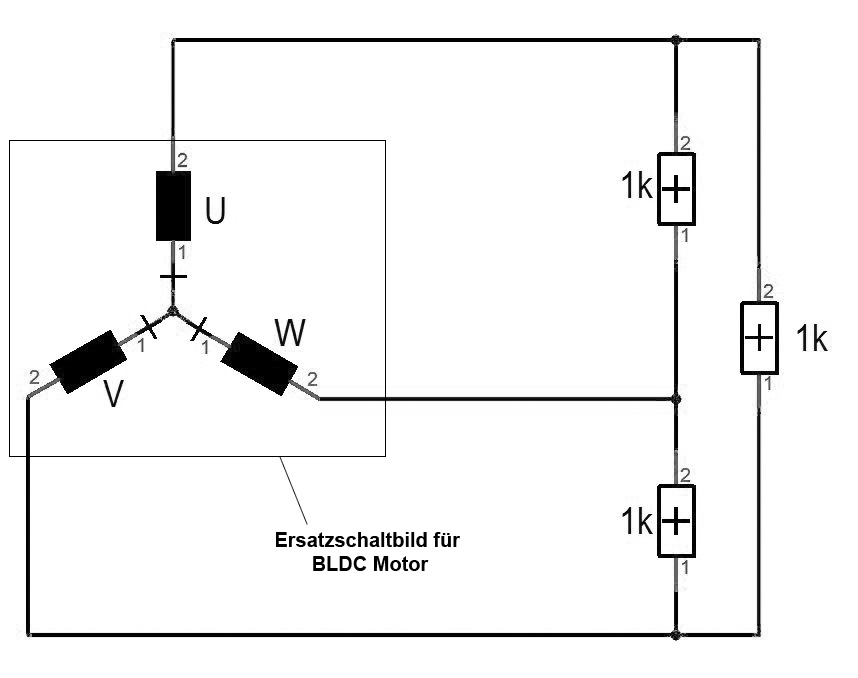
\includegraphics[width=8cm]{tests/graphics/Messchaltung_Fremderregung}
	\caption[Aufbau Spannungsmessung BLDC Motor]{Messaufbau zur Messung der \\generierten Spannung am BLDC Motor}
	\label{fig:BLDC_Fremderregung}
\end{figure}


Durch das erzeugen einer Drehbewegung, mittels einer an die Motorwelle angebrachten Bohrmaschine, wurde in den Spulen eine Spannung erzeugt.
In Abbildung \ref{fig:Spannungsmessung_BLDC_Motor} ist eine dieser Messungen dargestellt.
Im oberen Bereich ist der Anlauf gut zu erkennen.
Die Spannung an den Spulen U und V sind ca. 120 $^\circ$ zueinander verschoben.\\


Ebenso wurden die drei Hall-Sensoren des Motors und das Indexsignal eines Drehgebers, welcher an der Motorwelle befestigt ist, aufgezeichnet.
Weiterhin ist in der Abbildung zu sehen, dass die Flankenwechsel der Hall-Sensoren verschoben sind.
Es gibt dabei ein Muster von sechs Zuständen, welche die Hall-Sensoren bilden können.
Aus der Überlegung drei Signale, die jeweils zwei unterschiedliche Zustände annehmen könnte es den Anschein haben, dass es acht ($2^3$) Zustände sein sollten.
Dem ist jedoch nicht so. 
Es gibt keinen Zustand, bei dem alle Signalleitungen HIGH bzw. LOW sind. Dadurch fallen diese weg.
Im Detail ist zu erkennen, dass es 42 Flankenwechsel für eine Umdrehung notwendig sind.

\begin{figure}[htbp]
	\centering
	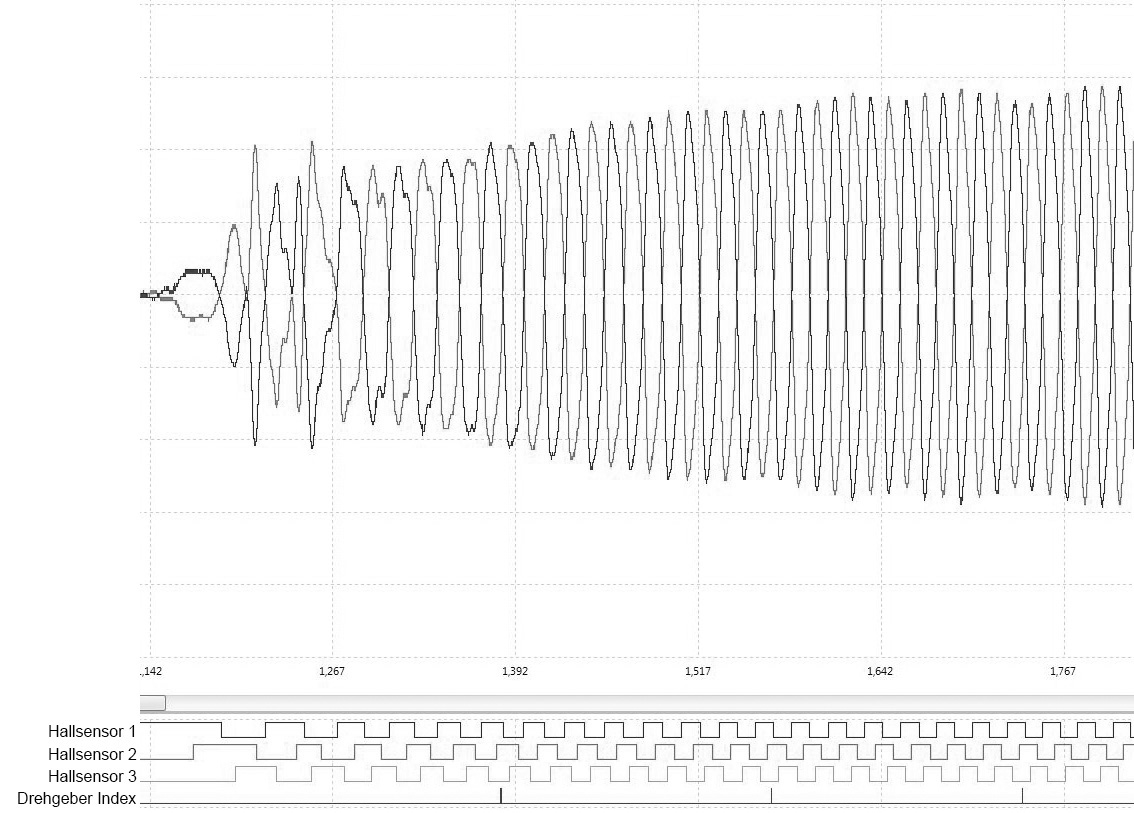
\includegraphics[width=\textwidth-2cm]{tests/graphics/Spannungssignal_Messung}
	\caption{Spannungsmessung BLDC-Motor}
	\label{fig:Spannungsmessung_BLDC_Motor}
\end{figure}


Doch jede Messung ist nur so gut wie Ihr Messaufbau.
Dies musste im auch bei diesem Aufbau festgestellt werden.
Für die Erzeugung der Drehbewegung wurde, wie eingangs erwähnt, eine Bohrmaschine verwendet.
Dabei handelt es sich um ein Gerät mit Anschlussleitung.\\


Abbildung \ref{fig:Fehlerbehaftete_Spannungsmessung_BLDC_Motor} zeigt das Messergebnis, welches mit der Messschaltung aus Abbildung \ref{fig:BLDC_Fremderregung} gemessen wurde.
Im Vergleich zu \ref{fig:Spannungsmessung_BLDC_Motor} zeigt dieses Bild Spannungsspitzen und Verzerrungen.
Die Störungen aus dem Analogsignal wurden durch Einstreuung auch auf die digitalen Signale der Hall-Sensoren übertragen.
Zu erkennen sind diese durch die vielen kleinen Spitzen.
Zuerst konnte der Fehler nicht gefunden werden.
Es wurde der Messaufbau neu erstellt, neue bzw. andere Messleitungen und sogar ein anderes Oszilloskop verwendet.
All diese Maßnahmen halfen jedoch nicht den Fehler zu beseitigen.
Es stellte sich heraus, dass die Anschlussleitung der Bohrmaschine bei diesen Messungen direkt über den Messleitungen verlief.
Dabei wurden Störungen, die durch den Gleichstrommotor in der Bohrmaschine entstanden sind, auf die Messleitungen übertragen.


\begin{figure}[htbp]
	\centering
	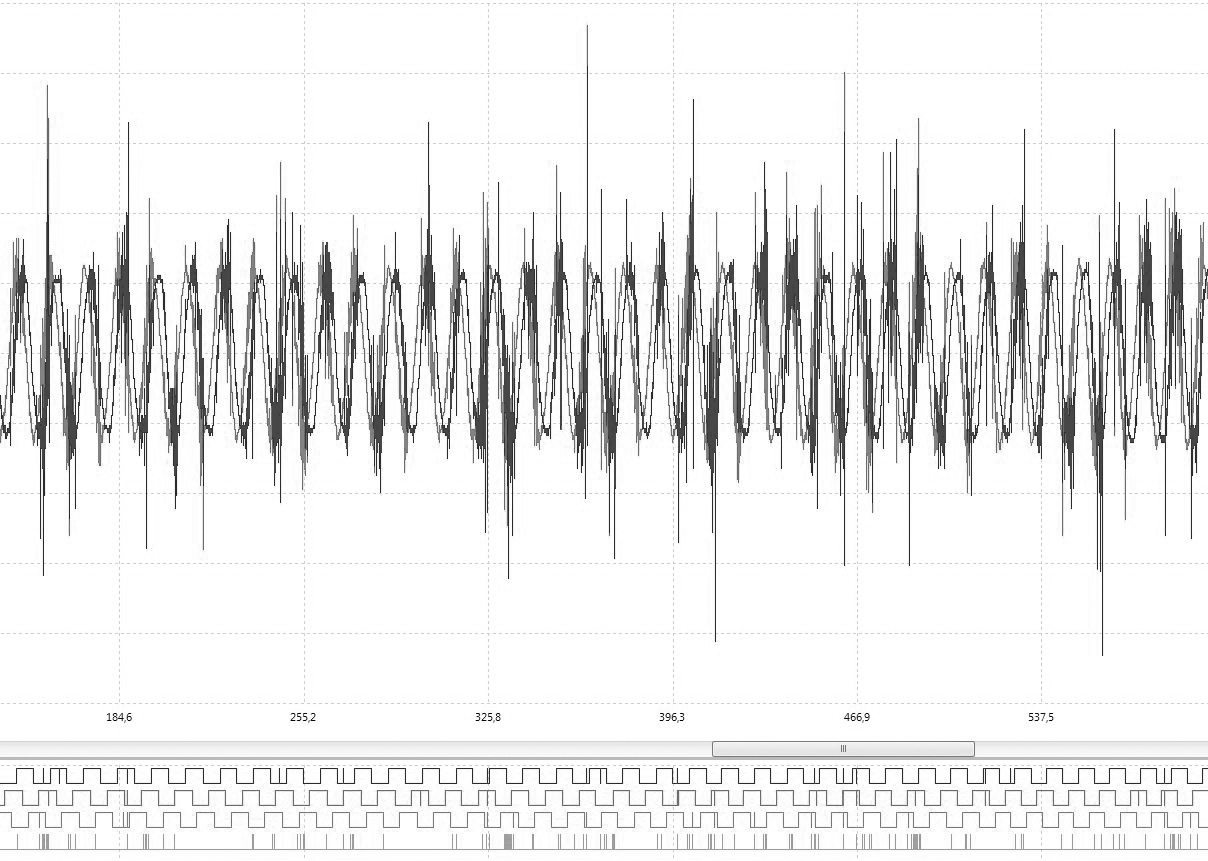
\includegraphics[width=\textwidth-2cm]{tests/graphics/Fehlerhaftes_Spannungssignal}
	\caption{Fehlerbehaftete Spannungsmessung BLDC-Motor}
	\label{fig:Fehlerbehaftete_Spannungsmessung_BLDC_Motor}
\end{figure}


\section{Hall-Sensorsignale in Verbindung mit dem XMC 4700 Relax Kit 5V}
Wie bereits im Abschnitt Hardware angedeutet hat es während des Projektverlaufs Probleme mit der Auswertung von digitalen Signalen in Verbindung mit dem XMC 4700 Relax Kit 5V gegeben.

Im Abschnitt \ref{sec:BLDC_mit_Fremderregung} sind in einigen Abbildungen die Signale der Hall-Sensor zu erkennen.
Diese wurden nur mit einem Oszilloskop aufgezeichnet.
Zur besseren Darstellung soll Abbildung \ref{fig:Hall_Sensor_OK} dienen.
Dort sind die verschiedenen Flankenwechsel gut zu erkennen.
Das Signal nimmt definierte Werte an und schwingt nicht.


\begin{figure}[htbp]
	\centering
	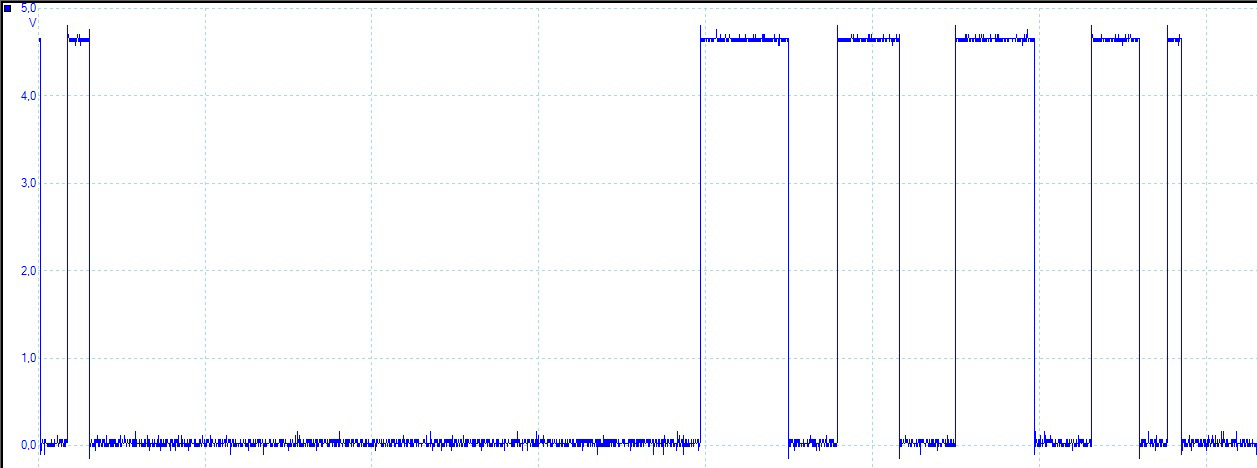
\includegraphics[width=\textwidth-4cm]{tests/graphics/hall_ok}
	\caption[Sensorsignal Hall-Sensor]{Sensorsignal eines Hall-Sensors}
	\label{fig:Hall_Sensor_OK}
\end{figure}

Dieses Signal veränderte sich jedoch als die Hall-Sensoren mit dem XMC 4700 Relax Kit 5V verbunden wurden.
Bild \ref{fig:Hall_Sensor_Fehlerhaft} zeigt das gemessenen Signal.
Gut zu sehen ist, dass es die Pegel nur bei LOW (0 Volt) einen definierten Wert annehmen.
Bei einem Wechsel auf HIGH (5 Volt) begann das Signal zu schwingen.
Nach mehreren Versuchen, dass Signal mit Kondensatoren zu stützen geriet der auf dem Relax Kit verbaute Pegelwandler in Verdacht.

Als Folge wurde das XMC 4700 Relax Kit 5V gegen ein XMC 4800 Relax EtherCat Kit ausgetauscht.
Dieses Board besitzt keine Pegelwandler.
Nach dem Austausch verschwand das Schwingen auf den Signalleitungen.

Der Hersteller der Pegelwandler, Texas Instruments, verweist mehrfach im Datenblatt des Pegelwandlers darauf die Signalleitungen so kurz wie möglich zu halten.
Auch auf den verschiedenen Supportseiten des Herstellers ist dieses Phänomen häufiger beschrieben.
Testweise wurden die Anschlussleitungen zwischen Hall-Sensoren und XMC 4700 Relax Kit 5V stark verkürzt.
Dadurch konnte das Schwingen eliminiert werden.

\begin{figure}[htbp]
	\centering
	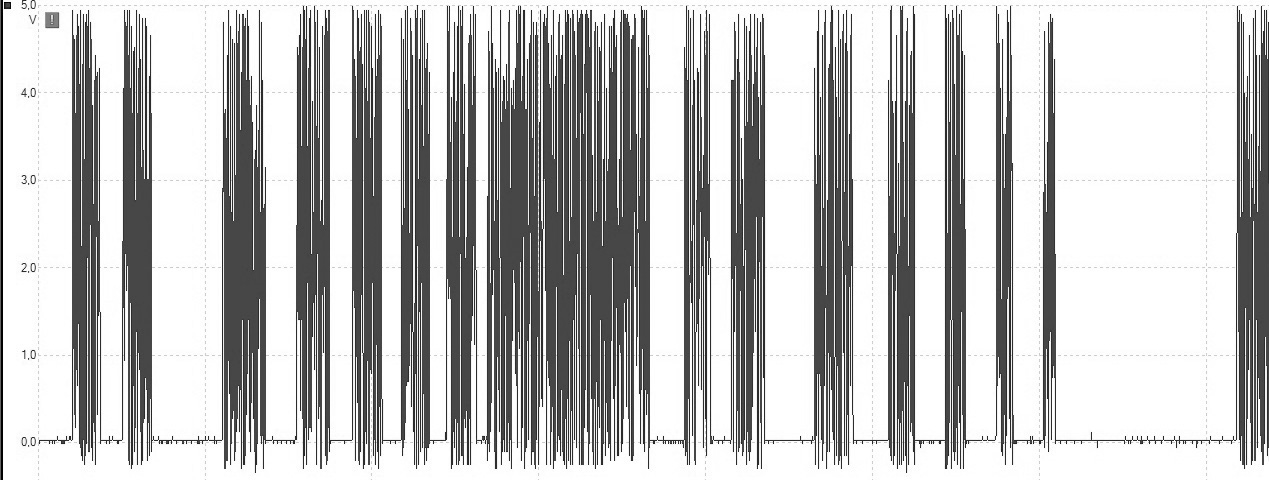
\includegraphics[width=\textwidth-4cm]{tests/graphics/hall_jitter_4700}
	\caption[Fehlerhaftes Sensorsignal eines Hall-Sensors]{Sensorsignal eines Hall-Sensors mit Störungen}
	\label{fig:Hall_Sensor_Fehlerhaft}
\end{figure}


\section{Steuersignale Relax Kit / H-Brücke}
Zur 



\section{Ansteuerungssignale Texas Instrument Evaluation Kit}

\section{Steuerungssignale }
